%Dokumentklasse
\documentclass[a4paper,12pt]{scrreprt}
\usepackage[left= 2.5cm,right = 2cm, bottom = 4 cm]{geometry}
%\usepackage[onehalfspacing]{setspace}
% ============= Packages =============

% Dokumentinformationen
\usepackage[
	pdftitle={Komplexe Leistung},
	pdfsubject={},
	pdfauthor={Lily Wagner},
	pdfkeywords={},	
	%Links nicht einrahmen
	hidelinks
]{hyperref}


% Standard Packages
\usepackage[utf8]{inputenc}
\usepackage[ngerman]{babel}
\usepackage[T1]{fontenc}
\usepackage{graphicx, subfig}
\graphicspath{{img/}}
\usepackage{fancyhdr}
\usepackage{lmodern}
\usepackage{color}
\usepackage{float}

%Punkte wegmachen
%\usepackage[titles]{tocloft}
%\renewcommand{\cftdot}{}




% Literaturverzeichnis
\usepackage[backend = biber,
			bibencoding = utf8,
			%style = ieee
			style = authoryear
			%style = authortitle,
			%style = alphabetic,
			]{biblatex}
\addbibresource{biblio.bib}

% Code
\usepackage{listings}

\definecolor{codegreen}{rgb}{0,0.6,0}
\definecolor{codegray}{rgb}{0.5,0.5,0.5}
\definecolor{codepurple}{rgb}{0.58,0,0.82}
\definecolor{backcolour}{rgb}{0.95,0.95,0.92}
\definecolor{burgundy}{rgb}{0.5, 0.0, 0.13}

\lstdefinestyle{Python}{
    language        = Python,
    basicstyle      = \ttfamily,
    keywordstyle    = \color{blue},
    stringstyle     = \color{codegreen},
    commentstyle    = \color{burgundy}\ttfamily
}

\lstset{
    frame       = single,
    numbers     = left,
    showspaces  = false,
    showstringspaces    = false,
    captionpos  = t,
    caption     = \lstname,
    tabsize 	  = 2,
    literate={\ \ }{{\ }}1
}

\def\inline{\lstinline[basicstyle=\ttfamily,keywordstyle={}]}

% zusätzliche Schriftzeichen der American Mathematical Society
\usepackage{amsfonts}
\usepackage{amsmath}

% nicht einrücken nach Absatz
\setlength{\parindent}{0pt}

% Automatische Absatz Abstand
\setlength\parskip{0.8em} 

% ============= Kopf- und Fußzeile =============
\pagestyle{fancy}
%
\lhead{}
\chead{}
\rhead{\slshape \leftmark}
%%
\lfoot{}
\cfoot{\thepage}
\rfoot{}
%%
\renewcommand{\headrulewidth}{0.4pt}
\renewcommand{\footrulewidth}{0pt}

% ============= Package Einstellungen & Sonstiges ============= 
%Besondere Trennungen
\hyphenation{De-zi-mal-tren-nung}


% ============= Table of Contents umdefinieren ================


% ============= Dokumentbeginn =============

\begin{document}
%Seiten ohne Kopf- und Fußzeile sowie Seitenzahl
\pagestyle{empty}

\begin{center}
\begin{tabular}{p{\textwidth}}


\begin{center}
%\includegraphics[scale=0.1]{img/logo.jpg}
\end{center}


\\

\begin{center}
\LARGE{\textsc{
Deadlocksanalyse unter der Betrachtung des Beispiels der Speisenden Philosophen von Dijkstra.
}}
\end{center}

\\


\begin{center}
\large{Städtisches Gymnasium Mittweida}
\end{center}

\\

\begin{center}
\large{Komplexe Leistung}\\
\end{center}


\begin{center}
\large{vorgelegt von}
\end{center}

\begin{center}
\large{{Lily Wagner}} \\
\end{center}

\begin{center}
\large{Klasse 10c}
\end{center}

\begin{center}
\large{Fachlehrer: Herr Schmidt}
\end{center}

\begin{center}
\large{30.09.2020}
\end{center}

\\

\\

\end{tabular}
\end{center}

% Beendet eine Seite und erzwingt auf den nachfolgenden Seiten die Ausgabe aller Gleitobjekte (z.B. Abbildungen), die bislang definiert, aber noch nicht ausgegeben wurden. Dieser Befehl fügt, falls nötig, eine leere Seite ein, sodaß die nächste Seite nach den Gleitobjekten eine ungerade Seitennummer hat. 
\cleardoubleoddpage

% pagestyle für gesamtes Dokument aktivieren
\pagestyle{fancy}

%Inhaltsverzeichnis
\tableofcontents



\chapter{Einleitung}
\label{sec:Einleitung}
Stellen Sie sich vor, Sie fahren auf einer Straße in ihrem Auto und gelangen an eine Kreuzung ohne Ampeln und Verkehrsschilder. Sie stehen mit vier weiteren Autos an dieser Kreuzung. In diesen Situationen gilt die Regel „rechts vor links“. Das bedeutet, dass kein Auto fahren darf, solange nicht das Auto rechts von ihm von der Stelle gefahren ist. Bestenfalls fahren zwei Autos gleichzeitig los und stoppen wieder, um einen Aufprall zu verhindern, das ist eine Frage der Koordination.
Abstrahiert man dieses Problem in die IT und ersetzt die Autos durch Prozesse, nennt man dies eine Verklemmung.
Die folgenden Seiten werden konkret das Problem der speisenden Philosophen genauer beleuchten.
Dieses Problem wurde als erstes 1965 von Djikstra formuliert und von dem selben auch gelöst. Seitem ist es ein beliebtes Beispiel zur Visualisierung bzw. Illustration von Verklemmungen und Deadlocks. Es ist eines der Worst-Case-Szenarios um Probleme in Algorithmen zu zeigen, in diesem Fall ist das Problem somit ein Deadlock.

Ein Beispiel eines Deadlocks gab es im Jahr 2019. Microsoft hatte ein Sammelupdate für Windows 10 herausgebracht, welches ein paar Probleme lösen sollte. Allerdings hatte sich bei Benutzern, die Windows 10 Version 1903 benutzten und das Update installierten, ein Prozess von Cortana verklemmt. Dabei kam es erst zu einer dauerhaften CPU-Auslastung von  ca 40 Prozent, da das Problem dann auftrat, wenn eine Anfrage an die Suchmaschine Bing von einer Methode wie einer Registry-Anfrage unterbunden wurde. Das Ergebnis dieses Deadlocks war, dass die Suchmaschine keine Suchergebnisse angezeigt hat.\parencite[vgl.][]{bug}

Es gibt unzählige Lösungen des Philosophen-Problems bis heute. 
Zu Anfang werden Grundlagen von Prozessen, Programmen sowie des Schedulings vorgestellt. Das darauf folgende Kapitel wird eine Verklemmung definieren, sowie die Bedingungen für eine solche erklären. 
Lösungsansätze werden vorgestellt, sowie Möglichkeiten gezeigt, wie eine Verklemmung visualisiert werden kann. Lösungsansätze einer Verklemungssituation sind die Themen des letzten Kapitels.
\chapter{Grundlagen}
\label{grundlagen}
\section{Erklärende Begriffe}
\label{sec:begriffe}
Ein Programm ist die Beschreibung eines mechanischen Rechenverfahrens, dass der Computer speichern und ausführen kann \parencite[vgl.][14]{rechenberg2000}. Vergleichbar ist dies mit einem Rezept. Wenn das Programm ausgeführt wird, nennt man es dann einen Prozess \parencite[vgl.][S.71]{tanenbaum2016}.Das Programm löst sozusagen einen Prozess aus. In der Analogie entspricht dies dem Koch, welcher das Rezept ausführt.  Dabei braucht ein Prozess auch “Zutaten”, um das Programm auszuführen, diese nennt den Betriebsmitteln. Das entspricht in der Realität zum Beispiel Arbeitsspeicher oder Dateien, Ressourcen, die beschrieben werden können. Es gibt wiederverwendbare Betriebsmittel oder konsumierbare Betriebsmittel. Die wiederverwendbaren Betriebsmittel werden von Prozessen belegt und nach deren Ausführung zur nächsten Verwendung  wieder freigegeben. Konsumierbare Betriebsmittel werden im laufenden System erzeugt (produziert) und anschließend zerstört (konsumiert).


Mit der Benutzeroberfläche des Betriebssystems, die Schnittstelle zwischen Hard- und Software, lässt sich beobachten, dass die Prozesse auf den Kernen des Prozessors sehr schnell wechseln. In wenigen Nanosekunden wechselt die CPU also zwischen den Prozessen umher, sodass zu einem Zeitpunkt nur ein Prozess läuft. Durch das schnelle Umschalten sieht es aus als würden mehrere Prozesse gleichzeitig laufen \parencite[vgl.][S.466]{sommer2002}. Damit  das funktioniert, wird ein Scheduler benötigt, welcher die Prozesse in eine Reihenfolge bringt und entscheidet welcher Prozess wann rechnen darf \parencite[vgl.][S.199]{tanenbaum2016}.

Es kann allerdings auch passieren, dass ein Scheduler selbst einen verklemmten Prozess weiter rechnen lässt, was allerdings zu keinem Ergebnis führt.
Wenn nun zwei Prozesse bereit zum Rechnen sind und um das gleiche Betriebsmittel konkurrieren und das Endergebnis der zwei Prozesse davon abhängt, welcher von den Prozessen als erstes rechnen darf, wird schnell der kritische Abschnitt erreicht. Der kritische Abschnitt umfasst \glqq die Teile des Programms, in denen auf gemeinsam genutzter Speicher zugegriffen wird'' \parencite[S. 164]{tanenbaum2016}. Wenn man diesen kritischen Abschnitt betritt, kommt es zu sogenannten Race Conditions. Race Conditions sind Situationen, \glqq in denen zwei oder mehr Prozesse einen gemeinsamen Speicher lesen oder beschreiben und das Endergebnis davon abhängt, welcher wann genau läuft'' \parencite[S. 166 f.]{tanenbaum2016}. Diese Situationen müssen vermieden werden wenn, von zwei Prozessen die gleiche Datei beschrieben werden soll und es davon abhängt wann welcher Prozess rechnen darf, zum Beispiel wenn ein Dokument bedruckt werden soll. Beschreiben zwei Prozesse das gleiche Dokument so kann es passieren kein inhaltlicher Zusammenhang mehr besteht. Verhindert werden kann dies mit wechselseitigem Ausschluss. Es kommt dann also gar nicht dazu, dass zwei Prozesse das gleiche Betriebsmittel verwenden bzw. gleichzeitig den kritischen Abschnitt betreten \parencite [vgl][S.471]{sommer2002}.

\section{Begriff Verklemmungen}
\glqq Eine Verklemmung (Deadlock)bezeichnet einen Zustand, in dem die beteiligten Prozesse wechselseitig auf den Eintritt von Bedingungen warten, die nur durch andere Prozesse aus dieser Gruppe selbst hergestellt werden können.'' \parencite[S.248]{sturm2001}. Diese wird durch Synchronisationsfehler erzeugt. 
Demnach macht keiner der Prozesse einen Fortschritt.

Es benötigt insgesamt vier Voraussetzungen damit letztendlich eine Verklemmung entsteht. Die erste ist der wechselseitige Ausschluss der Prozesse miteinander (engl. mutual exclusion). Dadurch ist ein Betriebsmittel unteilbar und exklusiv nutzbar. So werden zwar Race Conditions vermieden aber es besteht nun die Voraussetzung, dass zwei Prozesse nicht zur selben Zeit das gleiche Betriebsmittel verwenden können. Die Zweite ist das Nachfordern von den Betriebsmitteln ohne ein anderes loszulassen (engl. hold and wait). Die konkurrierenden Prozesse können nur schrittweise die Betriebsmittel belegen. Die dritte Bedingung besteht aus dem Fakt, dass einem Prozess die Betriebsmittel nicht entzogen werden können und nicht rückforderbar sind (engl. no preemption). Damit überhaupt eine Verklemmung vorliegen kann, müssen alle diese drei Bedingungen und eine Weitere eintreten. Diese vierte Bedingung heißt auf Englisch „circular wait“ und wird mit \textit{zirkuläres Warten} übersetzt. Deshalb muss es eine geschlossene Kette an wartenden Prozessen geben. Um zu einem Ergebnis zu kommen benötigt Prozess A das, was Prozess B erst herstellen muss und Prozess B, das was Prozess A erst noch herstellen muss. Also kommt es zu einem wechselseitigen kreisförmigen(zirkulären) Warten \parencite[vgl.][S. 195f.]{baun2017}.

Neben dem Deadlock, bei dem der Prozesszustand  \inline{BLOCKED} ist, gibt es auch noch den Livelock. Bei diesem ist der Prozesszustand \inline{RUNNING}, dabei führt die CPU den Prozess gar nicht aus da dieser mit einem anderen verklemmt ist. Der Livelock ist also wesentlich schwerer zu erkennen als der Deadlock \parencite[vgl.][S. 561 f.]{tanenbaum2016}.
\chapter{Die speisenden Philosophen}
\label{speisende_philosophen}
\section{Vorstellung des Modells}
\label{vorstellung}
Das 1965 von Dijkstra formulierte Philosophenproblem lässt sich wie folgt darstellen: Fünf Philosophen sitzen an einem runden Tisch. Jeder der Philosophen hat einen Teller mit Spagetti vor sich und weil die Nudeln so schlupfrig sind, benötigt man zwei Gabeln um sie zu essen. So liegt zwischen jedem Teller eine Gabel. Zusammengefasst gibt es nun fünf Teller mit den Spagetti und fünf Gabeln. Nun hat jeder Philosoph eine bestimmte Reihenfolge wie sie diese Tätigkeiten ausführen. Diese ist fest und unaustauschbar. Erst denken die Philosophen und weil Denken so hungrig macht, essen sie danach und heben erst die linke und dann die rechte Gabel auf. Dies kann auch lange gut gehen. Aber was passiert wenn alle Philosophen gleichzeitig hungrig sind und gleichzeitig nach der, von ihnen aus, linken Gabel greifen? Wenn jeder Philosoph nach seiner linken Gabel greift, hat keiner seine rechte Gabel. Also werden die Philosophen verhungern.\parencite[vgl.][S.220]{tanenbaum2016} 

\begin{figure}[H]
\caption{Modell \parencite{philosophers}}
\label{fig:modell}
\centering
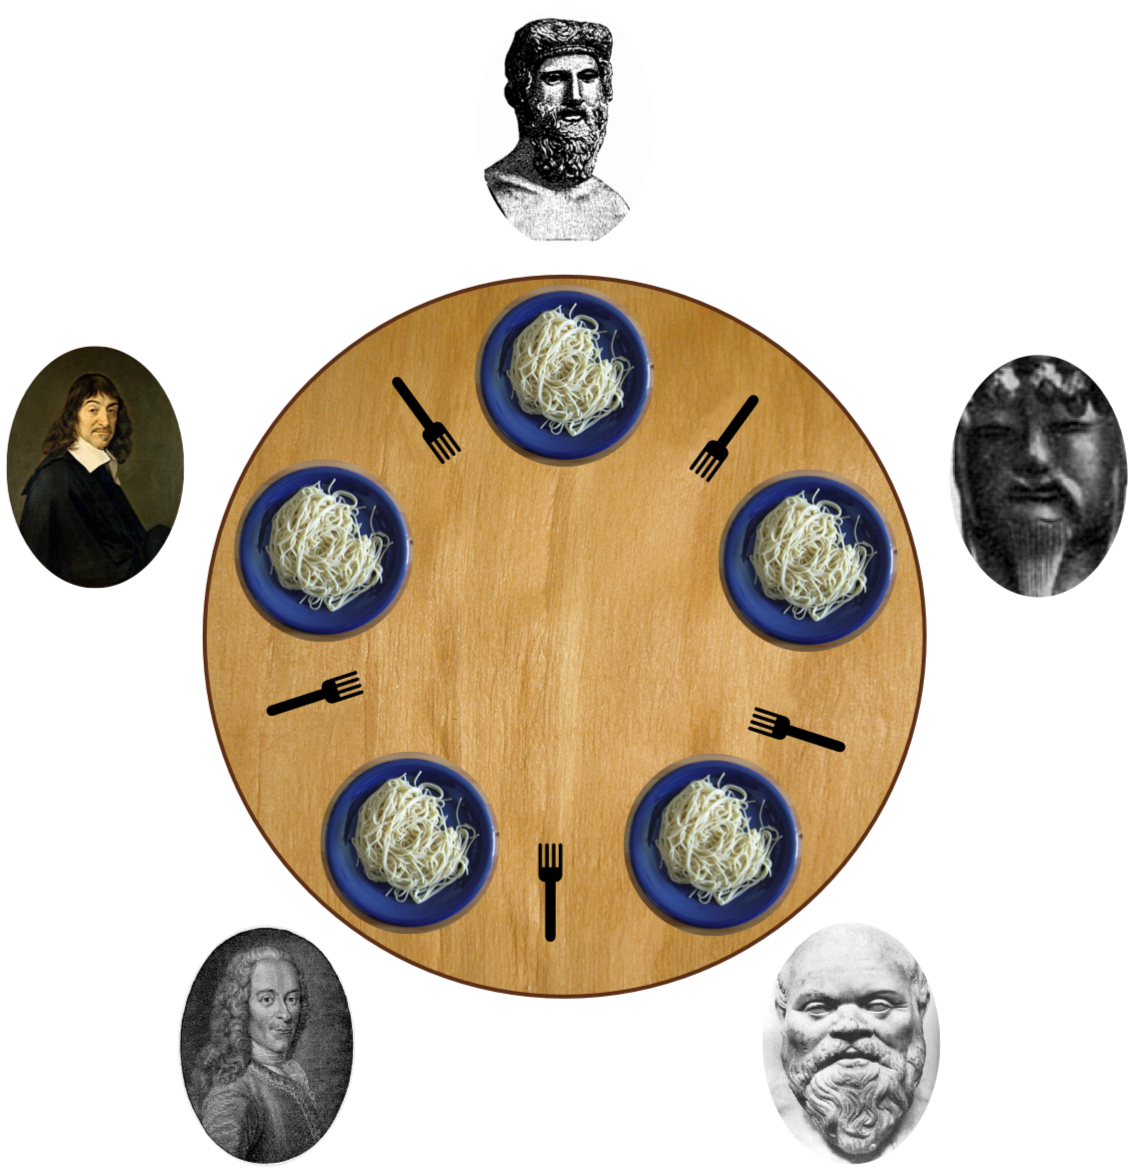
\includegraphics[width=.4\linewidth]{modell_dining_philosophers.png}
\end{figure}

Nun werden die Philosophen durch Prozesse ersetzt und die Gabeln durch Betriebsmittel und es kristalisiert sich eine Verklemmung heraus denn alle vier Bedingungen sind erfüllt. Mutual exclusion, da die Philosophen nicht zur selben Zeit mit der gleichen Gabel essen können. Hold and wait, da die Philosophen immer zuerst an sich denken und die Gabel keinem anderen überlassen. No preemption, die Philosophen sind gebildete Leute mit Manieren. Sie reißen einem anderem keine Gabel aus der Hand. Weil die Philosophen an einem runden Tisch sitzen und jeder auf die rechte Gabel wartet wird auch das Zirkuläre Warten erfüllt.

\section{Darstellung des Problems}
\label{problem}
Um das Problem ausfindig zu machen, gibt es verschiedene Möglichkeiten eine Verklemmung grafisch darzustellen. Um das Problem besser auflösen zu können, muss es erst sichtbar gemacht werden.

Vorgestellt wird zuerst der Betriebsmittelbelegungsgraph. Bei diesem werden die Prozesse mit Kreis und die Betriebsmittel mit Quadrat dargestellt. Diese werden ebenfalls als Knoten bezeichnet. Die Belegung und Anforderung auf Betriebsmittel wird mit Pfeilen, auch Kanten genannt dargestellt. Kommt dabei der Pfeil von dem Betriebsmittel zu dem Prozess, so bedeutet das, dass der Prozess dieses schon im Besitz hat. Verläuft der Pfeil von Prozess zu Betriebsmittel, so stellt der Prozess die Anforderung an das Betriebsmittel. Der Grundaufbau wird in Abbildung \ref{fig:normaler_betriebsmittelbelegungsgraph} gezeigt.

\begin{figure}[h]
\caption{Normaler Betriebsmittelbelegungsgraph}
\label{fig:normaler_betriebsmittelbelegungsgraph}
\centering
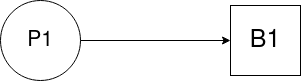
\includegraphics[width=.4\linewidth]{Belegungsgraph1.png}
\end{figure}

Bildet sich dabei eine zirkuläre Wartebeziehung so ist eine Verklemmung entstanden \parencite[vgl.][S. 197]{baun2017}.  In Abbildung \ref{fig:verklemmter_betriebsmittelbelegungsgraph} wird ein verklemmter Betriebsmittelbelegungsgraph dargestellt.
P1 besitzt Betriebsmittel B3 und benötigt B1. P2 hat Betriebsmittel B1 im Besitz und stellt die Anforderung an B2, welches schon von P3 belegt ist. P3 belegt B3 und fordert B1 an. Damit schließt sich der Kreis und es entsteht eine Verklemmung, da die vorhandenen Prozesse in einer zirkulären Wartebeziehung stehen.

\begin{figure}[H]
\caption{Bei diesem Beispiel liegt eine Verklemmung vor}
\label{fig:verklemmter_betriebsmittelbelegungsgraph}
\centering
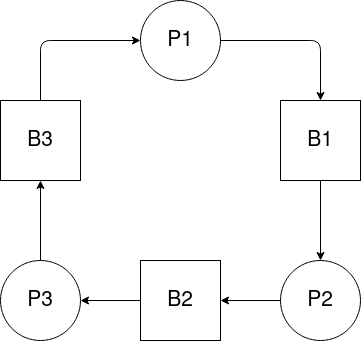
\includegraphics[width=.4\linewidth]{Belegungsgraph2.png}
\end{figure}

Eine andere Möglichkeit, eine Verklemmung darzustellen, ist das Prozess-Ablaufdiagramm. Bei letzterem werden die Prozesse auf der x- bzw. y-Achse dargestellt und deren Prozessfortschritt als Linie. Verläuft die Linie in y-Richtung, so rechnet P1, verläuft sie in x-Richtung rechnet P2. Die in dem Diagramm dargestellten ``Ecken'' symbolisieren die Änderung des Rechenvorgangs von P1 auf P2. Auf jeden der Achsen sind außerdem die angeforderten Betriebsmittel gekennzeichnet. Das orangene Feld kennzeichnet die Spanne wann ein Betriebsmittel belegt wird. In diesen Bereich können die Prozesse nicht hinein.
In Abbildung \ref{fig:normales_Ablaufdiagramm} wird ein normales Prozessablaufdiagramm ohne eine Verklemmung dargestellt.

\begin{figure}[H]
\caption{Möglicher Verlauf bei einem Prozessablaufdiagramm ohne Verklemmung}
\label{fig:normales_Ablaufdiagramm}
\centering
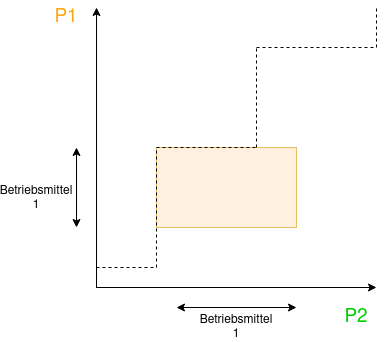
\includegraphics[width=.6\linewidth]{Prozess_Ablaufdiagramm.png}
\end{figure}

Nun wird ein zweites Betriebsmittel dazugenommen. Wie gewohnt rechnen die Prozesse, jedoch kann bei dem Beispiel \ref{fig:verklemmtes_ablaufdiagramm} eine Verklemmung entstehen. Die Zahlen 1-3 stellen mögliche Abläufe der Prozesse dar. Bei Ablauf 1 und 3 entsteht keine Verklemmung denn diese laufen jeweils links(1) und unterhalb(3) der gekennzeichneten Bereiche. Sie können ungehindert rechnen, denn sie belegen die Betriebsmittel, aber lassen diese anschließend wieder frei. Ablauf 3 jedoch gerät in den kritischen Abschnitt bis sich dann schließlich eine Verklemmung erkennen lässt. Verläuft die Linie des 3. Ablaufs weiter vertikal, so entsteht eine Verklemmung, denn Betriebsmittel 1 ist bereits von Prozess 1 belegt. Rechnet Prozess 1 weiter, so entsteht eine Verklemmung, denn Betriebsmittel 2 ist bereits von Prozess 2 bereits belegt ist. Zusammengefasst betritt die Linie 3 den roten Bereich, so ist eine Verklemmung unvermeidbar.
Eine Verklemmung ist bei einem solchen Diagramm nur möglich, wenn sich die Bereiche (in dieser Abbildung orange und grün gekennzeichnet) der Betriebsmittel so überschneiden, dass die Prozesse beide Betriebsmittel zur gleichen Zeit nutzen würden.

\begin{figure}[H]
\caption{Beispiel eines Prozessablaufdiagrammes mit Verklemmung}
\label{fig:verklemmtes_ablaufdiagramm}
\centering
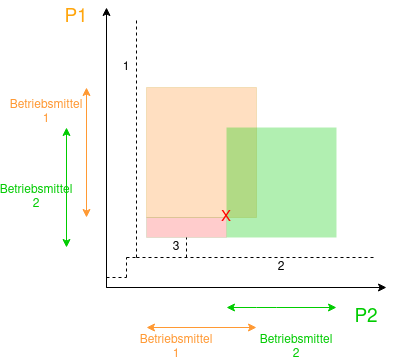
\includegraphics[width=.6\linewidth]{prozessablaufdiagramm2.png}
\end{figure}

\section{Lösungsansätze}
\label{sec:lösung}

Eine der möglichen Lösungen besteht daraus, das Problem zu ignorieren und einfach nichts zu tun. Das ist wahrlich eine sehr naive Lösung, die dennoch häufig benutzt wird, da sie ohne Aufwand für den laufenden Betrieb ist \parencite[vgl. ][S.79]{mandl2020} . Bei dieser Lösung terminieren jedoch die verklemmten Prozesse nicht.
 
Zur Vermeidung einer Verklemmung gibt es ebenfalls viele Möglichkeiten. Diese sind jedoch oftmals sehr  aufwendig. Auf unser Beispiel der speisenden Philosophen zurückkommend, besteht eine Lösung darin, eine vermittelnde Instanz zu erschaffen, welcher die Regeln bzw. den Ablauf für die Tätigkeiten der Philosophen auf den Tisch legt. Die Reihenfolge der Tätigkeiten der Philosophen wird genau festgelegt. Bei dieser Lösung kann bei fünf Gabeln nur ein Philosoph essen.\parencite[vgl.][S.220]{tanenbaum2016}

Die sinnvollste Lösung für ein solches Problem ist folgende: Die Philosophen müssen fragen, ob die linke Gabel frei ist. Ist die linke Gabel nicht frei, so denkt er weiter. Ist die linke Gabel frei, so fragt er nach der rechten Gabel. Ist diese nicht frei, legt er die linke Gabel wieder hin und denkt weiter. Erst wenn auch die rechte Gabel frei ist kann der Philosoph essen. Diese Lösung ermöglicht laut Tanenbaum \glqq ein Maximum an Parallelität für eine beliebige Anzahl von Philosophen.''\parencite[S.222]{tanenbaum2016}

Diese Lösung kann mithilfe von Sperren (engl. Lock) erreicht werden. Eine Sperre kann nur die Werte 1 oder 0 annehmen. Gilt der Wert der Sperre als 1, so ist diese belegt. Ist sie 0, dann nicht. Damit ein Prozess eine Sperre besetzen kann,  muss der Wert der Sperre 0 sein\parencite[vgl.][S.148]{mandl2020}.

Die Verklemmung kann allerdings auch von vornherein verhindert werden, indem das Eintreten der verklemmungsnotwenigen Bedingungen verhindert wird. Auch diese Lösung ist sehr aufwendig \parencite[vgl. ][S.79]{mandl2020}.


















\chapter{Programmierung}
\label{programmierung}

\section{Erste Lösung mit Problemdarstellung}
\label{erste_lösung}


\begin{lstlisting}[style = Python, label = {erste Lösung}, caption = {erste "naive" Lösung}]

from multiprocessing import Process, current_process, RLock
import time
import random


class Philosophers(Process):
    def __init__(self, name, leftFork, rightFork):
        print("{} Has sat down the table".format(name))
        Process.__init__(self, name=name)
        self.leftFork = leftFork
        self.rightFork = rightFork

    def run(self):
        print("{} has started thinking".format(current_process().name)) 
        #Philosoph x hat mit denken begonnen
        while True:
            time.sleep(random.randint(1, 5))
            print("{} has finished thinking".format(current_process().name))
            self.leftFork.acquire() 
            #philosoph x hat die linke Gabel
            time.sleep(random.randint(1, 5))
            try:
                print("{} has acquired the left fork".format(current_process().name))

                self.rightFork.acquire() 
                #Philosoph x hat die rechte Gabel
                try:
                    print("{} has attainted both forks, currently eating".format(current_process().name)) #Philosoph x hat beide Gabeln

                finally:
                    self.rightFork.release()
                    print("{} has released the right fork".format(current_process().name)) 
                    #Philosoph ist fertg mit essen und gibt die rechte Gable wieder frei

            finally:
                self.leftFork.release()
                print("{} has released the left fork".format(current_process().name)) 
                #Philosoph x hat gibt die linkte Gabel frei

\end{lstlisting}

In dem Programm werden die Bibliotheken "Multiprocessing" sowie "random" und "time" importiert. Die Klasse "Philosophers" erbt von der Klasse "Process" alle Funktionen und zusätzlich die, die in der Klasse "Philosophers" definiert werden. Zugleich kann ein Prozess losgetreten werden. Da sich die Philosophen über die gleichen Merkamle definjeren und sogesehen Objekte gleicher Kategorie sind können sie in einer kalsse zusammengefasst werden. Der Initialisierungsfunktion werden die Parameter \inline{name} sowie \inline{leftFork} und  \inline{rightFork}. Aus letzteren werden die Objekte leftFork und rightFork erzeugt. Diese stehen für die rechte- sowie linke Gabel. In der Zeit, in der der Philosoph denkt, schläft der Prozess(Programmzeile 18) repräsentativ. Der Zeitraum in der der Philosoph denken soll, wird zufällig zwischen einer und fünf Sekunden ausgewählt. Wenn der Philosoph fertig mit denken ist, fordert er die linke Gable an. Danach soll er versuchen die rechte Gabel zu bekommen. Hat er beide Gabeln so kann er essen. Ist er damit fertig, so kann er erst die rechte und dann die linke Gabel wieder freigeben.

Nun der Lösungsansatz hierbei ist, dass die Gabeln einen RLock repräsentieren. Das heißt die Prozesse besetzen immer Sperren. Um die Sperren zu besetzen, ruft der Prozess die aquire()-Funktion auf. Um sie wieder freizugeben ruft er die release()-Funktion auf. Diese "Lösung" ist jedoch nicht deadlockfrei. Wollen zwei Prozesse die gleiche Sperre besetzen so verklemmt das Programm sofort. 

\section{Lösungen}
\label{endlösung}

\begin{lstlisting}[style = Python, label = {mein_beispiel}, caption = {Das zeige ich euch}]



%\end{lstlisting}

Um diesem Problem vorzubeugen kann man der aquire()-Funktion entweder ein True oder ein False mitgeben. Die Funktion gibt True zurück, sollte der Lock besetzt sein, False falls nicht. Setzt man die Funktion auf True, so geht der Programmcode nicht weiter bis die Funktion ausgeführt ist, in diesem Fall wenn der Lock besetzt ist. Das heißt, will ein Prozess den Lock besetzen, so muss er immer wieder versuchen, diesen zu besetzen, bis dieser wieder freigegeben ist. Dieses Verfahren heißt blocking. 

\begin{lstlisting}[style = Python, label = {mein_beispiel}, caption = {Das zeige ich euch}]



%\end{lstlisting}


Der Prozess wird immer wieder versuchen die linke Gabel zu belegen, bis diese freigegeben ist. Dann soll er versuchen die rechte Gabel zu erlangen. Da dieser Lock auf False gesetzt ist, wird er das nur einmal versuchen. Geprüft werden kann dies an der Variable "locked". Scheitert dieser Versuch, so ist der Prozess nicht auf "locked" gesetzt und die linke Gabel wird wieder freigeben. Gelingt er, so kann man dies feststellen, da dann der Zustand des Prozesses auf locked gesetzt wird. Der Philosoph hat nun beide Gabeln, kann essen, dann die rechte und zuletzt auch die linke Gabel wieder freigeben. Nun kann der nächste Prozess wieder versuchen den Lock zu ergattern.
 








\chapter{Fazit}
\label{fazit}

Sie kann unter dem Modell der speisenden Philosophen veranschaulicht werden. Bei diesem Modell läuft es darauf hinaus, dass alle fünf Philosophen die von ihnen linke Gabel in der Hand haben und auf ihre rechte Gabel warten. Es entsteht eine sogenannte Verklemmung, zu Englisch ein Deadlock. Diese Verklemmung kann nur unter vier Bedingungen stattfinden. Es gibt verschiedene Arten eine Verklemmung zu visualisieren, wie zum Beispiel der Betriebsmittelbelegungsgraph. Dabei gibt es auch verschiedene Möglichkeiten auf eine Verklemmung zu reagieren. 

Der Deadlock kann ignoriert werden, wobei durch das Verklemmen der Prozesse diese nicht terminieren. Die Prozesse bleiben praktisch ergebnislos. 
Wenn die Verklemmung erkannt wurde, kann sie auch beseitigt werden.
Die Verklemmung kann auch vermieden sowie ausgeschlossen werden, indem der Eintritt einer der vier Bedingungen verhindert wird.

Es gab naive Lösungsansätze, die zumindest nicht verklemmen, allerdings den Effekt von paralleler Programmierung verlieren. 
In dem Programmbeispiel aus dieser Arbeit wurden jedoch die Gabeln durch Locks repräsentiert. Diese Lösung schafft ein Höchstmaß an Quasi-Parallelität und ist deadlockfrei. 

Diese Arbeit wurde unter Betracht eines Einprozessorsystems, wie in \ref{sec:begriffe} \nameref{sec:begriffe} dargestellt wurde, geschrieben. Mittlerweile gibt es Mehrprozessorsysteme, jedoch gilt auch dort das selbe Prinzip.

Weiterführend kann eine deadlockfreie Lösung des Problems durch Vermittler und Mutex Semaphoren geschaffen werden. 


\printbibliography[heading=bibintoc]


\cleardoublepage
% \phantomsection
\renewcommand{\listfigurename}{Materialienverzeichnis}

\addcontentsline{toc}{chapter}{\listfigurename}
%Verzeichnis aller Bilder
\listoffigures

%Verzeichnis aller Tabellen
\listoftables

\end{document}
